% Review variant. Preparation record retained in the companion repository.
% Author names, affiliations and email intentionally left blank at user request.
\documentclass{optica-article}
\journal{opticajournal}
\articletype{Research Article}
\usepackage{amsmath,booktabs}
% newtxmath already defines this symbol; let amsthm supply its proof marker.
\let\openbox\relax
\usepackage{amsthm}
\usepackage{iftex}
\ifXeTeX
\usepackage{fontspec}
\setsansfont{texgyreheros-regular.otf}[BoldFont=texgyreheros-bold.otf,ItalicFont=texgyreheros-italic.otf,BoldItalicFont=texgyreheros-bolditalic.otf]
\fi
\usepackage{lineno}
\linenumbers
\pagestyle{plain}
\newtheorem{theorem}{Theorem}
\newtheorem{proposition}{Proposition}
\begin{document}
\title{Response Tolerance and Spectral Regularity in Reference-Matched Reflectance Design}
\author{}
\address{}
\email{}
\begin{abstract*}
Response tolerance changes the capacity cost of spectral regularity. We study passive reflectances that match a flat 50\% reference under D65 and approximate a prescribed transformation under A and FL11. At global effect-relative XYZ tolerance 0.10, the capacity gain beyond unchanged-spectrum target inflation is over 50\% larger with derivative bounds than with passivity alone. Exact certificates prove strict gain ordering over a tolerance interval for both named-illuminant and all-mixture constraints. Every feasible derivative-bounded design at or above a certified attainable amplitude exceeds that class's exact X-response limits for the same transformation under A and FL11, with a necessary Y deficit under A.
\end{abstract*}
\thispagestyle{plain}

\section{Introduction}
A passive material can match a reference under one illuminant and produce a different color response under another. Designing that difference requires a single reflectance spectrum to satisfy several response constraints simultaneously. Spectral regularity further restricts the available spectra. An exact response specification and an approximate one can therefore incur different costs from the same regularity constraint. The question addressed here is whether a fixed response allowance can recover more absolute transformation capacity in a regularity-constrained class than it adds to the unrestricted passive class.

The ingredients of this problem have substantial precedents. Metamer sets describe the spectra sharing a specified response~\cite{Finlayson2005}. Smoothest reflectance reconstruction selects among such spectra through a regularity objective~\cite{vanTrigt1990,Burns2020}. Li and Luo combined reference matching, passivity, multi-illuminant color inconstancy, and spectral smoothness~\cite{Li2006}; Li \emph{et al.} developed a reflectance-based color gamut using related constraints~\cite{Li2007}. Paramer formulations admit response neighborhoods and permit spectral gamut mapping across multiple illuminants~\cite{Urban2011,Morovic2021}. These approaches establish the relevance of approximate matching and regularized spectral design. The Li--Luo formulations seek low multi-illuminant inconstancy subject to reflectance and smoothness conditions. Here the transformation direction is fixed, and the objective is its maximum attainable amplitude at a specified error allowance. We compare the resulting absolute capacity increments in two nested spectral classes.

Recent operator treatments describe color formation through kernels, quotient spaces, and physically constrained response sets~\cite{Morovic2026Quotient}, and express metamer mismatching and limits of linear chromatic adaptation through a residual operator~\cite{Morovic2026Mismatch}. Those results characterize information loss and prediction between viewing conditions. Our design problem fixes the response transformation and optimizes a passive spectrum that preserves a reference match. Its central comparison concerns how spectral regularity changes the additional amplitude made available by response tolerance.

Regularity also changes the extent of object-color and mismatch sets. Flinkman \emph{et al.} used derivative statistics to construct a smoothness-restricted object-color solid~\cite{Flinkman2012}. Stiebel and Merhof examined the effect of allowing unrealistic spectral roughness in metamer-mismatch models~\cite{Stiebel2017}. Such restrictions reduce the set of attainable responses. Set inclusion alone, however, does not determine which of two nested spectral classes gains more capacity when a response tolerance is introduced.

We compare these increments in common absolute units. The capacity is the largest amplitude of a fixed response transformation that one spectrum can implement while retaining an exact reference match. A nonzero tolerance permits an elementary increase in nominal target amplitude without any change to the spectrum. Subtracting this unchanged-spectrum contribution isolates a further capacity bonus. We prove that, for the specified D65/A/FL11 problem, this bonus is more than 50\% larger under a first-derivative envelope than under passivity alone. The unrestricted class still has greater total capacity. Thus regularity carries a capacity penalty, while the allowed error reduces that penalty by a provably positive amount.

The response consequences are established separately from the target-amplitude comparison. At or above a certified attainable amplitude, every feasible regularity-constrained design exceeds the actual X increment of every exact design in the same derivative-bounded class for the prescribed transformation under both additional illuminants. Every such design also incurs a positive Y deficit under A. These universal bounds identify a benefit and a necessary cost of the high-capacity regime, beyond the behavior of one computed spectrum.

The analysis uses support inequalities and exact feasibility certificates, drawing on standard convex methods~\cite{Boyd2004}. Its contribution is the quantitative relation between spectral regularity, absolute tolerance benefit, and actual multi-illuminant response. The upper bounds cover measurable or absolutely continuous reflectances on the full wavelength interval. The lower bounds are explicit spectra. Together they establish the conclusions without requiring a numerical optimizer to locate an exact extremum.

\section{Reference-matched spectral design}
\subsection{Response model and spectral classes}
Let $I=[380,780]$ nm and let $r:I\to[0,1]$ be a passive, nonfluorescent reflectance. Write $z=r-1/2$ for its displacement from the flat reference. For illuminant $j$, define
\begin{equation}
 A_j z=\int_I f_j(\lambda)z(\lambda)\,d\lambda,
 \qquad c_j=A_j1,
 \label{eq:response}
\end{equation}
where $f_j$ is the three-component illuminant--observer response kernel. The actual tristimulus vector is $c_j/2+A_jz$.

We use the CIE 1931 $2^\circ$ observer and illuminants D65, A, and FL11~\cite{CIEObserver,CIED65,CIEA,CIEFL}. Each source function is specified by piecewise-linear interpolation of the frozen tabulated values on the 1 nm grid. Illuminant--observer products are therefore piecewise quadratic and are integrated as products. Each illuminant is scaled so that the perfect diffuser has $Y=100$. The model treats the interpolated functions as its exact inputs; this convention is especially relevant to the structured FL11 spectrum. Supplement 1 gives the source identifiers, normalization, and certificate representation.

The unrestricted class and the derivative-bounded class are
\begin{align}
 \mathcal U&=\{z\in L^\infty(I): |z|\leq1/2\ \text{a.e.}\},\label{eq:U}\\
 \mathcal S&=\{z\in AC(I): |z|\leq1/2,\ \ell\leq z'\leq u\ \text{a.e.}\},\label{eq:S}\\
 \ell&=-0.0094\ \mathrm{nm}^{-1},\qquad u=0.0244\ \mathrm{nm}^{-1}.\nonumber
\end{align}
The first-derivative endpoints are those reported for the combined derivative-value distribution in Table 1 of Ref.~\cite{Flinkman2012}. Here they define a fixed sensitivity class. We impose no curvature bound. Coverage of derivative values in a source collection does not imply coverage of the same proportion of complete material spectra.

\subsection{Transformation and illumination domain}
Use index $0$ for D65, $1$ for A, and $2$ for FL11. The primary transformation is
\begin{equation}
 H_X=\begin{pmatrix}1&-c_{0,X}/c_{0,Y}&0\\0&0&0\\0&0&0\end{pmatrix},
 \qquad h_j=H_Xc_j.
 \label{eq:HX}
\end{equation}
At amplitude $\beta\geq0$, the target is $c_j/2+\beta h_j$. Equation~\eqref{eq:HX} annihilates the reference white exactly. Under another illuminant it prescribes an X change proportional to the difference between that illuminant's X/Y ratio and the D65 ratio, while retaining the target Y and Z. One common spectrum must implement the responses under every specified condition.

We consider either the three named illuminants or all their nonzero nonnegative mixtures. For the latter, homogeneity permits weights $w_j\geq0$ with $\sum_jw_j=1$, and
\begin{equation}
 A_w=\sum_jw_jA_j,\quad c_w=\sum_jw_jc_j,\quad h_w=\sum_jw_jh_j.
 \label{eq:mixture}
\end{equation}
Separate positive rescaling of the generating illuminants preserves their mixture cone. Let $\mathcal J$ denote the selected illumination domain and set
\begin{equation}
 K=\max_{w\in\mathcal J}\frac{\|h_w\|_2}{\|c_w\|_2}.
 \label{eq:K}
\end{equation}
For these inputs, exact Gram inequalities establish the same $K$ for the named and mixture domains. No automatic transfer from named-lamp errors to mixture errors is assumed.

\subsection{Fidelity, capacity, and the inflation correction}
Fix $0\leq\rho<1$. A feasible design in class $\mathcal C\in\{\mathcal U,\mathcal S\}$ satisfies
\begin{equation}
 z\in\mathcal C,\quad A_0z=0,\quad
 \|A_wz-\beta h_w\|_2\leq\rho\beta K\|c_w\|_2
 \quad(w\in\mathcal J).
 \label{eq:contract}
\end{equation}
Its capacity is
\begin{equation}
 b_{\mathcal C}(\rho)=\sup\{\beta\geq0:\text{Eq.~\eqref{eq:contract} is feasible}\}.
 \label{eq:capacity}
\end{equation}
For $\beta>0$, the fidelity criterion is the ratio
\begin{equation}
 J(z,\beta)=\frac{\displaystyle\max_{w\in\mathcal J}
 \|A_wz-\beta h_w\|_2/\|c_w\|_2}
 {\displaystyle\max_{w\in\mathcal J}
 \|\beta h_w\|_2/\|c_w\|_2}\leq\rho.
 \label{eq:relative}
\end{equation}
We choose $\rho=0.10$ as the primary computational criterion. It compares maxima over illumination conditions. It is neither a 10\% error relative to each illuminant's individual target change nor a perceptual threshold.

\begin{proposition}[Unchanged-spectrum baseline]\label{prop:baseline}
Let $K>0$ and $0\leq\rho<1$. If $z$ is exact for the prescribed transformation at amplitude $\beta_0\geq0$, then, for $\beta>0$,
\begin{equation}
 J(z,\beta)=\frac{|\beta-\beta_0|}{\beta}.
 \label{eq:inflationexact}
\end{equation}
For $\beta\geq\beta_0$, the same spectrum is feasible exactly when $\beta\leq\beta_0/(1-\rho)$. Consequently the supremum of amplitudes achievable by retaining an exact spectrum in class $\mathcal C$ is $b_{\mathcal C}(0)/(1-\rho)$.
\end{proposition}
\begin{proof}
Exactness gives $A_wz=\beta_0h_w$. The numerator of Eq.~\eqref{eq:relative} is $|\beta-\beta_0|K$ and the denominator is $\beta K$. For $\beta\geq\beta_0>0$, solving $1-\beta_0/\beta\leq\rho$ gives the stated condition. If $\beta_0=0$, no positive amplitude satisfies it for $\rho<1$. Taking the supremum over exact spectra proves the last statement, including the zero-amplitude case.
\end{proof}
This elementary baseline accounts for target inflation with an unchanged material. We define the additional capacity bonus by
\begin{equation}
 \Delta_{\mathcal C}(\rho)=b_{\mathcal C}(\rho)-\frac{b_{\mathcal C}(0)}{1-\rho}\geq0.
 \label{eq:bonus}
\end{equation}
Both classes use the same transformation and amplitude scale. Their bonuses can be compared directly, without division by different exact capacities. Multiplication by $K$ expresses the same comparison in maximum incident-normalized intended-change units, $\alpha=K\beta$.

Geometrically, impose the D65 equality and map the remaining spectra to their joint A/FL11 response vectors. Exact capacity is the furthest intersection of this attainable set with the ray $\beta(h_1,h_2)$. Tolerance replaces the point on the ray by a surrounding admissible region whose size grows with $\beta$; mixture constraints further restrict this region. Inclusion of attainable sets orders total capacities but does not order their tolerance increments. The asymmetric derivative envelope of $\mathcal S$ does not give it central symmetry.

The nine response moments have full rank, verified by an exact rational minor. Positive exact designs exist in both classes. The capacities are finite for $\rho<1$: at an illumination attaining $K$, the triangle inequality gives $(1-\rho)\beta\|h_w\|_2\leq\|A_wz\|_2$, and passivity bounds the right side. Weak-star compactness for $\mathcal U$ and uniform compactness for $\mathcal S$ also give attainment. These properties justify the capacity comparisons independently of a finite-dimensional optimization model.

\section{Certificates for the full spectral classes}
\subsection{Support bounds and feasible spectra}
For multiplier vectors $\mu_j\in\mathbb R^3$, define
\begin{equation}
 g=\sum_{j=0}^2\mu_j^{\mathsf T}f_j,\quad
 P=\sum_{j=0}^2\mu_j^{\mathsf T}h_j,\quad
 W\geq\sum_{j=1}^2K\|c_j\|_2\|\mu_j\|_2.
 \label{eq:dual}
\end{equation}
The D65 error is zero. Every feasible spectrum obeys
\begin{equation}
 \beta(P-\rho W)\leq\int_Igz.
 \label{eq:support}
\end{equation}
For $\mathcal U$, $\int_Igz\leq\tfrac12\int_I|g|$. If $P-\rho W>0$, this gives an upper capacity bound. Rational Bernstein enclosures evaluate the absolute integrals of the piecewise-polynomial kernels.

For $\mathcal S$, two bounds are used. The exact-response bound starts from a support inequality for the endpoint interpolant $Lz$ and adds a continuous-function correction. On a unit wavelength bin, let $g(t)=a+bt+ct^2$. Then
\begin{align}
 \int_0^1g(t)[z(t)-Lz(t)]\,dt&=\int_0^1K_P(s)z'(s)\,ds,\\
 K_P(s)&=\frac a2+\frac b6+\frac c{12}-as-\frac b2s^2-\frac c3s^3.
 \label{eq:peano}
\end{align}
Since $\int_0^1K_P=0$, the absolute correction is at most $(u-\ell)\int_0^1|K_P|/2$. The interpolant retains passivity and slope bounds. Its reference response need not be exact, because the finite inequality being transferred is a support bound, not a feasibility assertion.

The tolerant upper bound uses a continuous piecewise-cubic function $\phi$ that vanishes at both ends of $I$. Integration by parts yields
\begin{equation}
 \int_Igz\leq\frac{u-\ell}{2}\int_I|\phi|
 -\frac{u+\ell}{2}\int_I\phi+\frac12\int_I|\phi'-g|.
 \label{eq:ibp}
\end{equation}
Equations~\eqref{eq:peano} and~\eqref{eq:ibp} establish upper bounds for the entire absolutely continuous class.

A witness is an explicit feasible spectrum. Lower bounds use piecewise-linear witnesses with exact rational node values. The verifier checks the passive box, every slope, the reference moments, and the response inequalities. Optimizer termination is not used as a feasibility or optimality certificate. Supplement 1 provides the support constructions and the arithmetic needed to reproduce the enclosures.

\subsection{Certification for all illuminant mixtures}
For a proposed witness, write $e_j=A_jz-\beta h_j$. The matrices
\begin{equation}
 G_{ij}=K^2c_i^{\mathsf T}c_j-h_i^{\mathsf T}h_j,
 \qquad
 Q_{ij}=\rho^2\beta^2K^2c_i^{\mathsf T}c_j-e_i^{\mathsf T}e_j
 \label{eq:grams}
\end{equation}
are checked entrywise. Nonnegative entries imply $w^{\mathsf T}Gw\geq0$ and $w^{\mathsf T}Qw\geq0$ for every nonnegative $w$. A named illumination attains $K$, so the target certificate proves Eq.~\eqref{eq:K} for the whole mixture domain. The error certificate proves witness feasibility there. Upper bounds using named conditions also bound the smaller all-mixture feasible set. Consequently the capacity enclosures below apply to both illumination domains, without asserting that their exact capacities are equal.

\section{Absolute tolerance benefit}
\begin{theorem}\label{thm:main}
For the inputs, transformation, and spectral classes in Sec.~2, and for either illumination domain, the following statements hold:
\begin{enumerate}
\item At $\rho=0.10$, $\Delta_{\mathcal U}>0$ and
\begin{equation}
 \Delta_{\mathcal S}>1.50\,\Delta_{\mathcal U}.
 \label{eq:mainresult}
\end{equation}
\item $\Delta_{\mathcal S}(\rho)>\Delta_{\mathcal U}(\rho)$ throughout $[0.056736,0.137809]$.
\item $b_{\mathcal S}(\rho)<b_{\mathcal U}(\rho)$ at $\rho=0$ and $0.10$, while
\begin{equation}
 [b_{\mathcal S}(0.10)-b_{\mathcal S}(0)]-
 [b_{\mathcal U}(0.10)-b_{\mathcal U}(0)]>0.0355394472.
 \label{eq:rawgain}
\end{equation}
\end{enumerate}
\end{theorem}

\begin{proof}
The support and feasibility certificates give Table~\ref{tab:capacity}. Lower and upper endpoints are combined in opposite directions when subtracting capacities. Exact rational arithmetic gives
\begin{align}
 0.1614029983&<\Delta_{\mathcal S}(0.10)<0.2528752265,\\
 0.0866515534&<\Delta_{\mathcal U}(0.10)<0.1075820401.
 \label{eq:bonusbounds}
\end{align}
The ratio of the certified lower S endpoint to the certified upper U endpoint exceeds $1.50027828$. Positivity of the lower U endpoint proves Eq.~\eqref{eq:mainresult}. The same four capacity enclosures establish the strict total-capacity ordering and Eq.~\eqref{eq:rawgain}.

For the interval statement, let $r=0.10$, let $b_0,b_1$ be the exact and tolerant S witness amplitudes, and set $k=(b_1-b_0)/(rb_1)$. Convex blending of these witnesses gives
\begin{equation}
 b_{\mathcal S}(x)\geq\frac{b_0}{1-kx}\quad(0\leq x\leq r).
 \label{eq:blend}
\end{equation}
For $r\leq x<1$, the same tolerant spectrum gives $b_{\mathcal S}(x)\geq(1-r)b_1/(1-x)$. A fixed unrestricted support gives $b_{\mathcal U}(x)\leq L/(P-Wx)$. Use $B_0\geq b_{\mathcal S}(0)$ and $U_0\leq b_{\mathcal U}(0)$ from the certificates. Below $r$, positivity of the bonus difference follows from
\begin{multline}
 b_0(P-Wx)(1-x)-L(1-kx)(1-x)\\
 +(U_0-B_0)(1-kx)(P-Wx)>0.
 \label{eq:intervalpolynomial}
\end{multline}
Above $r$, the corresponding numerator is $[(1-r)b_1+U_0-B_0](P-Wx)-L(1-x)$. All denominators are positive over the stated interval. Exact coefficient and endpoint signs prove positivity of the quadratic below $r$ and the decreasing affine numerator above $r$. Supplement 1 gives the constants and sign checks.
\end{proof}

\begin{table}[htbp]
\centering
\caption{Certified capacity enclosures. Display endpoints are rounded outward. Exact rational certificates determine all strict comparisons.}
\label{tab:capacity}
\begin{tabular}{lcc}
\toprule
Class and tolerance & Lower bound & Upper bound\\
\midrule
$\mathcal U$, $\rho=0$ & 0.3817259867 & 0.3835151503\\
$\mathcal U$, $\rho=0.10$ & 0.5127794981 & 0.5317220254\\
$\mathcal S$, $\rho=0$ & 0.2101706137 & 0.2171923873\\
$\mathcal S$, $\rho=0.10$ & 0.4027278731 & 0.4863981307\\
\bottomrule
\end{tabular}
\end{table}

\begin{figure}[htbp]
\centering
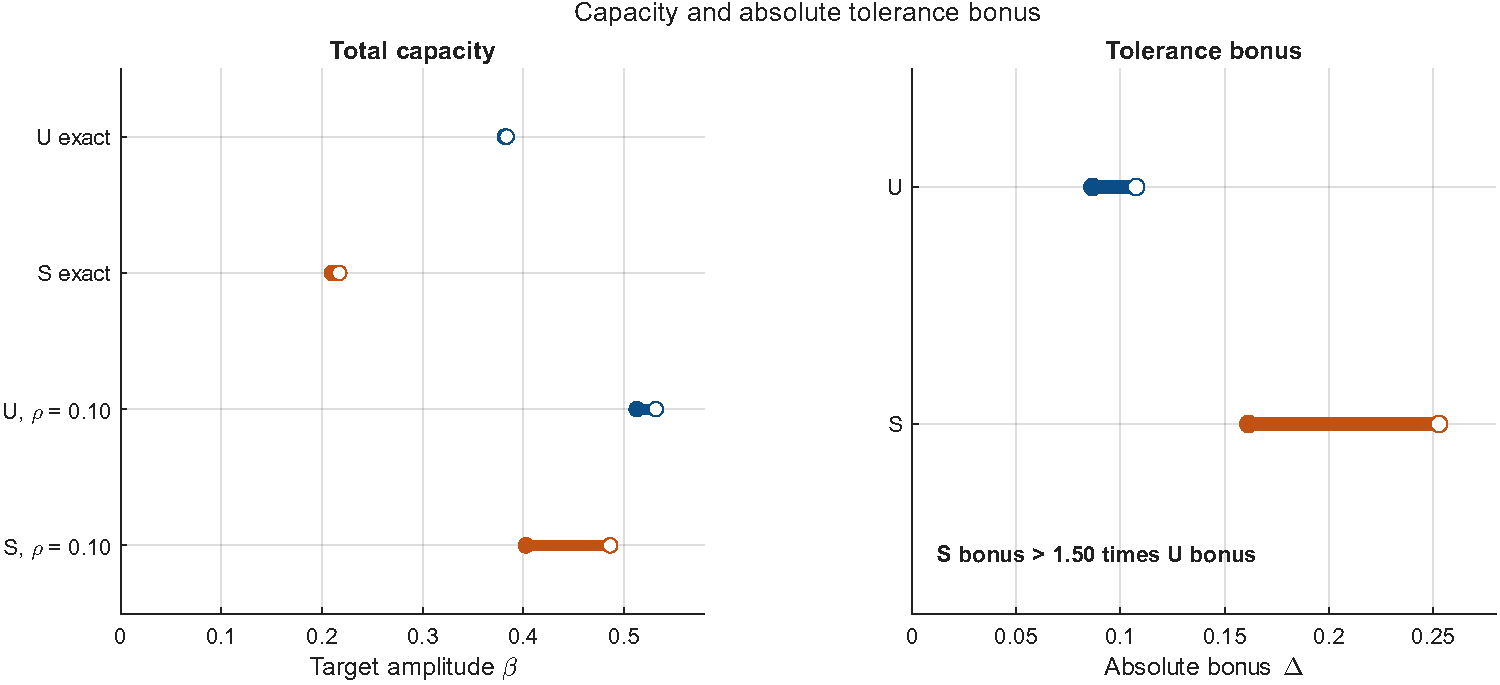
\includegraphics[width=\linewidth]{figures/01-capacity-and-absolute-bonus.pdf}
\caption{Capacity and absolute tolerance bonus for the two spectral classes. Filled endpoints are certified lower bounds; open endpoints are full-class upper bounds. Each segment is an enclosure, not a confidence interval. Regularity lowers total capacity at both tolerances, while its lower bonus bound exceeds 1.50 times the unrestricted upper bonus bound. Plotted endpoints summarize the exact certificates.}
\label{fig:capacity}
\end{figure}

The capacity enclosures in Fig.~\ref{fig:capacity} give a positive regularity penalty $d(\rho)=b_{\mathcal U}(\rho)-b_{\mathcal S}(\rho)$ at both endpoints. The bonus difference satisfies the identity
\begin{equation}
 \Delta_{\mathcal S}(\rho)-\Delta_{\mathcal U}(\rho)
 =\frac{d(0)}{1-\rho}-d(\rho).
 \label{eq:penaltyidentity}
\end{equation}
Thus bonus ordering alone compares $d(\rho)$ with the inflated penalty $d(0)/(1-\rho)$. The separate raw-increment inequality~\eqref{eq:rawgain} proves that $d(0.10)<d(0)$. The endpoint calculation in Supplement 1, Sec.~4.A, gives
\begin{equation}
 \frac{d(0)-d(0.10)}{d(0)}>0.2160.
 \label{eq:penalty}
\end{equation}
Thus the allowance removes more than 21.60\% of the exact-response penalty. The absolute intended-X bonus has the same ordering: under A the S lower bound is 2.38984110, whereas the U upper bound is 1.59293188; under FL11 the corresponding bounds are 0.95451625 and 0.63622614. These are target-bonus units with white $Y=100$. Actual responses are considered in Sec.~5.

\begin{figure}[htbp]
\centering
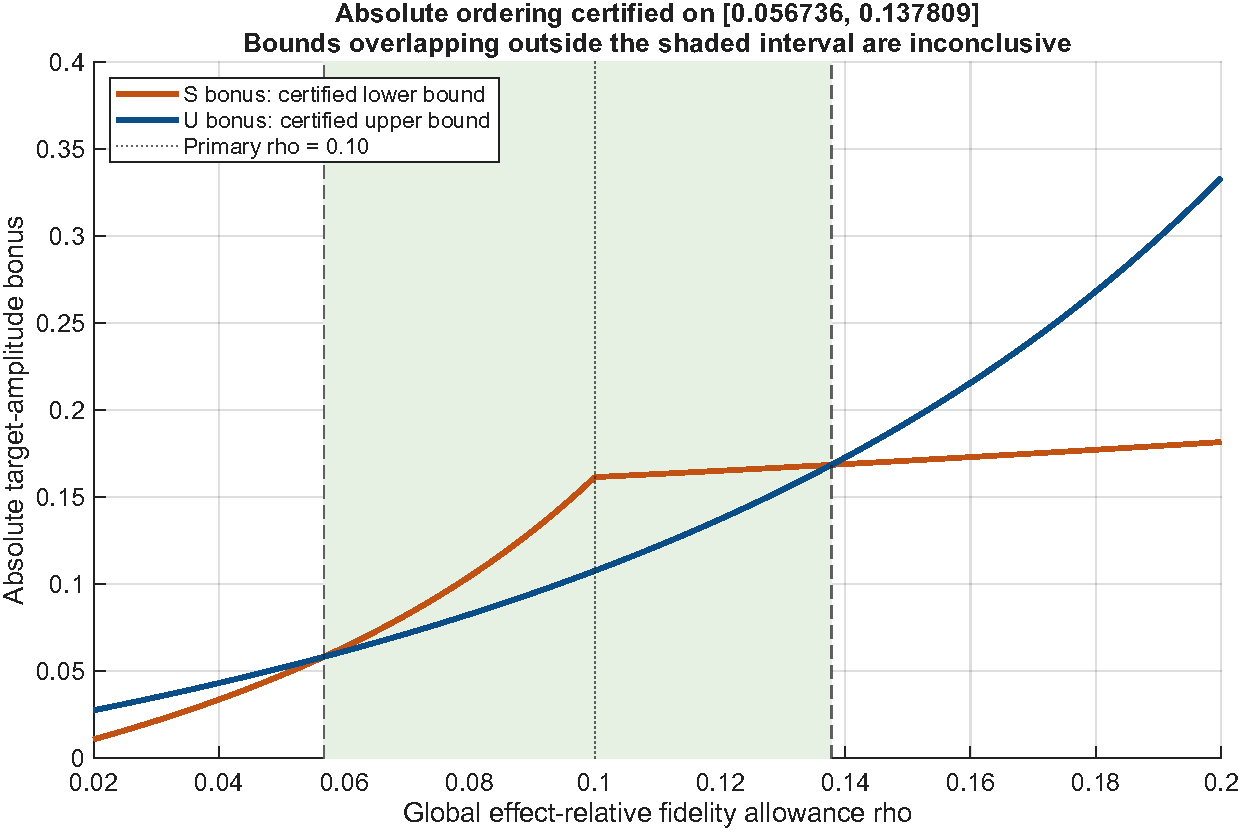
\includegraphics[width=0.96\linewidth]{figures/02-tolerance-interval.pdf}
\caption{Analytical lower bound for the S bonus and upper bound for the U bonus. The certified strict-ordering interval is $[0.056736,0.137809]$. Its proof uses polynomial signs over the full interval; sampled curve points are only a visualization. The endpoints are sufficient bounds and do not identify the actual crossings.}
\label{fig:interval}
\end{figure}

The interval in Fig.~\ref{fig:interval} shows that the comparison persists across a range of allowances around the primary value. At the sensitivity values 0.05 and 0.20, the available absolute-bonus bounds overlap. They do not determine the ordering at those two values.

\section{Actual response gains and a necessary Y cost}
Let $\beta_*\simeq0.4027278731222646$ denote the exact rational amplitude of the certified tolerant S witness. This amplitude is attainable for the named conditions and for all their nonnegative mixtures. Figure~\ref{fig:cost} compares the witness responses with the universal bounds proved below.

\begin{theorem}\label{thm:response}
Every feasible $z\in\mathcal S$ at $\rho=0.10$ and $\beta\geq\beta_*$ satisfies
\begin{align}
 (A_1z)_X&>5.44012708, & (A_2z)_X&>1.77273816,\label{eq:actual}\\
 (A_1z)_Y&<-0.24083547.\label{eq:Ycost}
\end{align}
Every exact S design for the prescribed transformation has X increments below 3.21589624 under A and 1.28444742 under FL11. The actual-X improvements in Eq.~\eqref{eq:actual} therefore exceed 69.1636\% and 38.0156\%, respectively. If an additional condition $(A_1z)_Y\geq0$ is imposed, every feasible amplitude obeys $\beta<0.2679937276830<\beta_*$.
\end{theorem}

\begin{proof}
Use the exact-baseline S multipliers and their full-class support bound $L_{\mathcal S}=P_{\mathcal S}B_0$. With $e_j=A_jz-\beta h_j$, Eq.~\eqref{eq:support} before the error-ball estimate gives
\begin{equation}
 \sum_j\mu_j^{\mathsf T}e_j\leq L_{\mathcal S}-\beta P_{\mathcal S}.
\end{equation}
Eliminating the other secondary lamp's error ball leaves, for lamp $j$,
\begin{equation}
 \mu_j^{\mathsf T}e_j\leq B_j=L_{\mathcal S}-\beta C_j,
 \quad\|e_j\|_2\leq T_j=\beta\rho K\|c_j\|_2,
 \label{eq:cap}
\end{equation}
where $C_j=P_{\mathcal S}-\rho K\|c_{3-j}\|_2\|\mu_{3-j}\|_2$ for $j=1,2$. For a unit coordinate vector $a$, put $p=a^{\mathsf T}\mu_j$ and $s^2=\|\mu_j\|_2^2$. The maximum of $a^{\mathsf T}e$ over this ball intersected with a half-space is $T_j$ if $pT_j\leq B_j$; otherwise, for a nonempty cap, it is
\begin{equation}
 \frac{pB_j+\sqrt{s^2-p^2}\sqrt{s^2T_j^2-B_j^2}}{s^2}.
 \label{eq:capformula}
\end{equation}
Apply this expression to $a=-e_X$ and $a=e_Y$, enclosing each radical outward. At $\beta_*$ the resulting bounds give Eqs.~\eqref{eq:actual} and~\eqref{eq:Ycost}. After division by $\beta$, the cap shrinks as $\beta$ grows because $L_{\mathcal S}/\beta$ decreases. The positive normalized X lower bounds and negative normalized A-Y upper bound therefore extend to all larger feasible amplitudes. Exact designs have $(A_jz)_X\leq B_0h_{j,X}$, which gives the comparison values. Restricting the A error ball further to $e_{1,Y}\geq0$ gives the stated amplitude upper bound. Details and rational enclosures appear in Supplement 1.
\end{proof}

\begin{figure}[htbp]
\centering
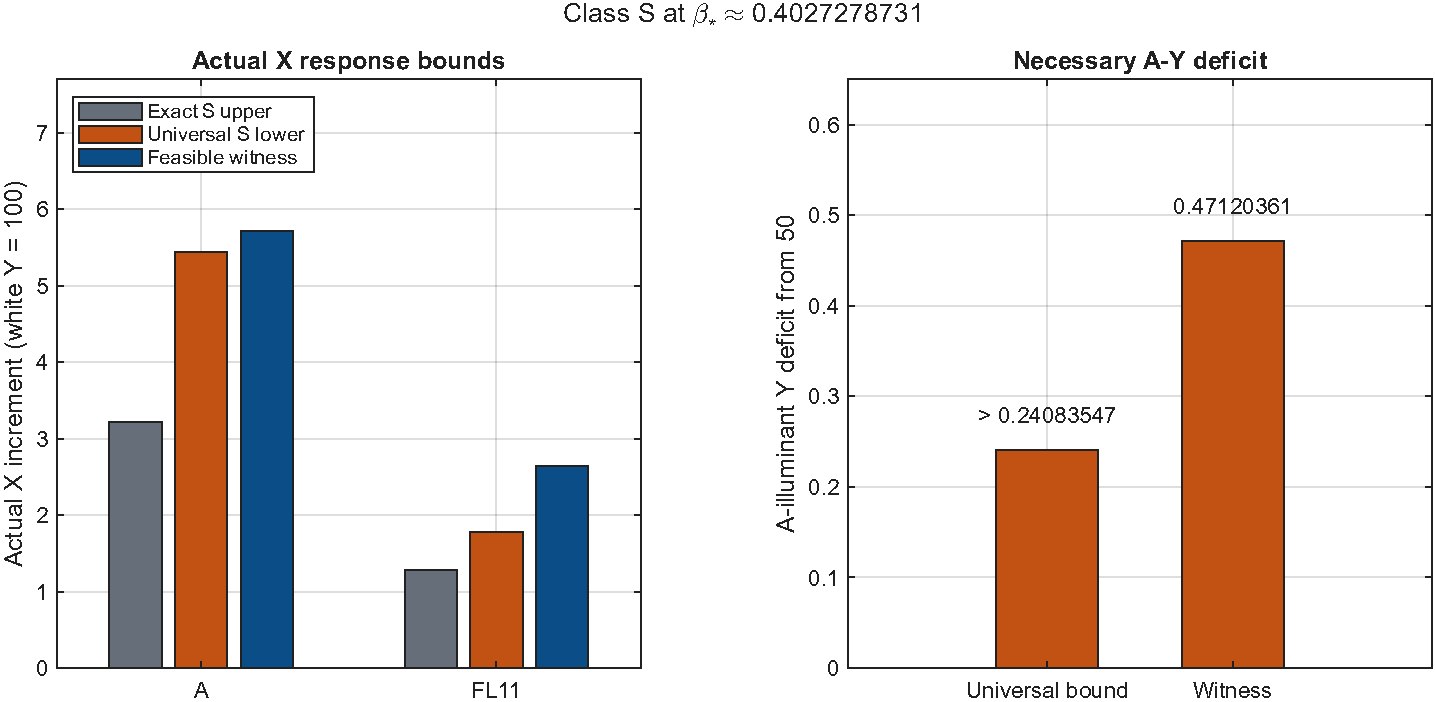
\includegraphics[width=\linewidth]{figures/03-actual-response-and-cost.pdf}
\caption{Actual response consequences at $\beta\geq\beta_*$. Universal lower X bounds apply to every feasible S design in this regime and exceed the exact S upper bounds for the same prescribed transformation. Witness values describe one attainable spectrum. The A-Y deficit is necessary. The analysis does not establish a positive necessary FL11-Y deficit. All values are tristimulus increments or deficits relative to the flat 50\% reflector, with white $Y=100$.}
\label{fig:cost}
\end{figure}

\begin{table}[htbp]
\centering\small
\caption{Absolute response quantities for the certified S witness at $\beta_*$. D65 target, actual change, and error are exactly zero. Entries for the other illuminants are rounded display values. $\eta_j=\|e_j\|_2/(\beta_*K\|c_j\|_2)$ is the lamp's contribution to the global criterion.}
\label{tab:response}
\begin{tabular}{lrr}
\toprule
Quantity & A & FL11\\
\midrule
Intended X increment & 5.96305915 & 2.38168005\\
Actual X increment & 5.72070507 & 2.64286342\\
Actual Y increment & $-0.47120361$ & $-0.55000421$\\
Actual Z increment & 0.27351857 & $-0.00942588$\\
X error & $-0.24235407$ & 0.26118336\\
Y error & $-0.47120361$ & $-0.55000421$\\
Z error & 0.27351857 & $-0.00942588$\\
Absolute error $\|e_j\|_2$ & 0.59630591 & 0.60894189\\
Global-normalized contribution $\eta_j$ & $<0.10$ & $<0.10$\\
\bottomrule
\end{tabular}
\end{table}

Under FL11, the witness error in Table~\ref{tab:response} is about 25.6\% of that lamp's intended X change, while its contribution to Eq.~\eqref{eq:relative} remains below 10\%. Reporting the absolute errors alongside the declared global normalization makes this distinction explicit. Equation~\eqref{eq:Ycost} is a signed tristimulus result: the A response has $Y<49.75916453$. It is not a prediction of perceived brightness. The comparator consists of exact $\mathcal S$ designs for $H_X$.

\section{Direction and model sensitivity}
The same exact reference permits the fixed direction
\begin{equation}
 H_Z=\begin{pmatrix}0&0&0\\0&0&0\\0&-c_{0,Z}/c_{0,Y}&1\end{pmatrix}.
\end{equation}
To compare directions in common units, let $\Phi_d=K_d\Delta_{\mathcal S,d}(0.10)$. Exact lower and upper certificates give
\begin{equation}
 \Phi_X>0.0156453680148,\quad
 0\leq\Phi_Z<0.0003455399445,\quad
 \Phi_X>45.278\,\Phi_Z.
 \label{eq:direction}
\end{equation}
This inequality includes a zero Z bonus. It compares two prescribed directions, with no optimization over directions. The construction and figure are in Supplement 1.

A separate norm comparison uses one invertible linear map $D$ consistently for the error, target, and incident XYZ vectors. Writing $\kappa=\operatorname{cond}_2(D)$, norm equivalence bounds the normalized error by factors $\kappa^{-2}$ and $\kappa^2$. The saved capacity certificates then prove
\begin{equation}
 \Delta_{\mathcal S,D}(0.10)>\Delta_{\mathcal U,D}(0.10)
 \quad\text{if}\quad 1\leq\kappa\leq1.052918.
 \label{eq:norm}
\end{equation}
This is a sufficient radius for the X class comparison. Equation~\eqref{eq:direction} is established in the original Euclidean norm; the two conclusions are separate.

Two analytical properties further specify the result's scope. First, both classes have the same capacity suprema as their $C^\infty$ subclasses when no common higher-derivative bound is imposed. Strict contraction, positive mollification, and a finite-dimensional moment correction preserve the prescribed responses and spectral inequalities. Thus the capacity comparison does not depend on piecewise-linear corners. Second, capacities are continuous under sufficiently small $L^1$ perturbations of the response kernels, with continuous reference-annihilating targets, preserved moment rank, positive incident norms, and fixed derivative bounds. The strict bonus ordering consequently persists in a neighborhood of the specified input functions. Supplement 1 proves both statements. They establish equality of suprema and qualitative stability, respectively; they do not supply smooth endpoint attainment or a numerical input-uncertainty radius.

\section{Discussion}
The distinction between total capacity and tolerance benefit changes the interpretation of spectral regularity. At exact fidelity, the derivative envelope imposes a substantial capacity penalty. At the selected tolerance, the restricted class remains smaller, but it gains more absolute capacity. Removing unchanged-spectrum inflation makes this comparison informative even when the exact capacities differ substantially. The certified factor above 1.50 cannot be explained solely by expressing the improvement as a percentage of a smaller regularized baseline.

The actual-response theorem gives the capacity comparison a concrete colorimetric meaning. Every feasible $\mathcal S$ design operating at $\beta_*$ or above exceeds the exact prescribed-transform X limits of $\mathcal S$ under both A and FL11. Under A it must also surrender some Y. The response allowance therefore changes which combinations of intended effect and collateral response are feasible. A design brief that additionally requires no A-Y loss excludes the certified high-capacity regime, even though it uses the same exact D65 reference. This conclusion applies to every feasible design in the stated class and regime.

Earlier reconstruction and paramer methods construct spectra subject to smoothness, response equality, and tolerance constraints. The present comparison asks how the absolute capacity increment differs between two nested spectral classes when the same allowance is introduced. The certificate bounds answer that question for a fixed transformation and connect it to necessary actual responses. Optimization, response neighborhoods, and derivative constraints are established tools. The result quantifies their interaction for the full spectral classes of the chosen model.

The study's application is reference-matched spectral design under specified illumination. Its coordinates, derivative envelope, and effect-relative tolerance are explicit design choices. A particular pigment system, printing process, or coating family would add its own realization constraints. A perceptual specification would require a corresponding perceptual error model. Such changes define further design problems; the present certificates give a reproducible baseline against which their capacity costs can be assessed.

\section{Conclusion}
For passive reflectances preserving the response of a flat 50\% reflector under D65, a response allowance can be more valuable under spectral regularity in absolute terms. In the specified CIE 1931/D65/A/FL11 model, the derivative-bounded class has an inflation-corrected capacity bonus more than 50\% larger than the unrestricted passive class at $\rho=0.10$. The strict ordering holds throughout a certified tolerance interval and for all nonnegative mixtures of the three illuminants. Every feasible derivative-bounded design at or above a certified attainable amplitude produces larger actual X increments than every exact design in the same class for the prescribed transformation, with a necessary A-Y deficit. These results quantify how fidelity and regularity jointly determine attainable response changes.

\begin{backmatter}
\bmsection{Funding}
% Intentionally blank: to be supplied by the author.
\bmsection{Disclosures}
% Intentionally blank: the author must supply the conflict-of-interest declaration.
\bmsection{Data availability}
The exact input fixture, certificate verifier, MATLAB figure code, and tabulated results are included in the accompanying \texttt{reproducibility/} package. The CIE source datasets are identified in Refs.~\cite{CIEObserver,CIED65,CIEA,CIEFL}. A public release location has not been assigned.
\bmsection{Supplemental document}
See Supplement 1 for detailed proofs, certificate construction, sensitivity calculations, and reproduction instructions.
\end{backmatter}
\bibliography{references}
\end{document}
